\chapter{Polynomial Classes and Genomics}
\label{chap:polyclass}


  This chapter examines the so called \emph{polynomial classes}, those
  permutation classes whose enumeration is given by a polynomial for large
  enough sizes. Much research in the area of permutation classes focuses on
  characterizing exponential growth rates, with a particular
  focus on the principally based classes. Considerably less attention has been
  paid to the small permutation classes~\cite{Vatter2011,Vatter2010} of which the
  polynomial classes, having subexponential growth, are an example. 

  These classes have recently found biological applications to the field of
  genomics. Evolution and mutation of organisms can be modelled as a
  rearrangement of a sequence of genes, and permutations have recently been
  applied to model these rearrangements~\cite{GenomeBook}. The physical
  mechanics of genome rearrangement have led to a variety of operations on
  permutations, and the theory of geometric grid classes~\cite{GridClasses}
  provides a geometric foundation from which to study these various operations.
  The polynomial classes are a subset of these grid classes, and arise when
  modelling the evolutionary distance. 

  Polynomial classes can characterized in a number of ways, but determining the
  actual polynomial which enumerates such a class can be computationally
  difficult. While there are several established methods for enumerating
  permutation classes, many of these are inefficient and none take advantage of
  the inherent structure in these classes.  In this chapter, we introduce an
  algorithm which quickly and efficiently enumerates a polynomial class from a
  structural description of the class.  This allows for an extension of
  existing genomic data, as well as a framework for further investigation. This
  chapter is based in part on~\cite{me-polyclass}, and the algorithm,
  implemented in Python, is freely available online~\cite{polyclass-algo}. 
  


% =========================================================================== %
\section{Class Structure}
\label{polyclass:sec:gridclasses}
% =========================================================================== %

  \begin{definition} \label{polyclass:def:polyclass}
    A permutation class $\C$ is a \emph{polynomial class} if and only if the
    function $p(n) = |\C_n|$ is given by a polynomial for large enough $n$. 
  \end{definition} 

  It is not obvious that this definition gives way to a strict geometric
  description, as we shall soon see. Geometric grid classes provides a range of
  tools for analyzing the geometric properties of permutation class structure,
  and has produced new enumerative techniques for classes. To describe
  polynomial classes, however, we don't need the full machinery of geometric
  grid classes; these classes can be defined entirely using inflations
  (Definition~\ref{prelim:def:inflation}). 

  Note first that the polynomial classes fall under the purview of several
  established approaches, which could \emph{theoretically} be used to enumerate
  the classes~\cite{GridClasses, RegInsEnc, Atkinson2005, Linton2005,
  Brignall2008}. However, each of these approaches has its own drawbacks, and
  none provides an enumeration directly from a structural description of the
  class. Further, the work presented here illuminates some of the preliminary
  obstacles preventing a similar algorithmic approach to geometric grid
  classes. 
  


  \subsection{Peg Permutations}

    Polynomial classes can be viewed by considering a set of restricted
    inflations of a finite set of permutations. In order to properly analyze
    these inflations, we introduce an additional structure on permutations which
    will be used to specify which inflations are allowed. 

    \begin{definition} \label{polyclass:def:pegperm}
      A \emph{peg permutation} $\tro$ is a permutation $\ro = \ro_1 \ro_2 \dots
      \ro_n$ in which each entry is decorated with either a $+$, $-$, or
      $\bullet$. The \emph{length} of a peg permutation $\tro$ is just the
      length of the underlying permutation $\ro$. 
    \end{definition}
    
    For example, $ \tro = \pl3 \mn1 \dt2 \pl4$ is a peg permutation of length $4$,
    and there are $3^n n!$ peg permutations of length $n$. 
    We denote peg permutations with a tilde, while the underlying permutation
    (with decoration removed) is written without.

    We allow peg permutations to be inflated with \emph{monotone} intervals. The
    entries marked with a $+$ (resp. $-$) can be inflated with ascending (resp.
    decreasing) runs. Entries marked with a $\blt$ can be inflated with a single
    entry. Note that we go against tradition and allow empty inflations. It
    follows then that such an inflation can be described simply as a peg
    permutation together with a sequence of integers which represent the number of
    elements by which to inflate each entry. We formalize this below. 

    \begin{definition} \label{polyclass:def:inflation}
      Let $\tro = \tro_1 \tro_2 \dots \tro_n$ be a peg permutation of length
      $n$, and $\vec i = (i_1, i_2, \dots i_n)$. Then let $\tro(I)$ be the
      permutation obtained by inflating entry $\tro_k$ by an interval of size
      $i_k$ according to the decoration of $\tro_k$: an ascending run if the
      decoration is a $+$, a descending run if it is a $-$, and a single entry if
      a $\blt$. If $\tro_k$ has a dot, then $i_k$ must be $0$ or $1$, otherwise
      $i_k \in \Zgeq$. 
    \end{definition}

    
    Recall, for example, the class $\Av(123, 231)$ examined in
    Section~\ref{prelim:sec:av123+231}. The decomposition of this class was
    shown in Figure~\ref{prelim:fig:polygrid}, and can be described as
    inflations of the peg permutation $\pl 3 \pl 1 \pl 2$. 

    Like many definitions in this dissertation, this one is best illustrated with
    a graphic example. Figure~\ref{polyclass:fig:inflation} shows a peg
    permutation being inflated and then standardized into a permutation. The
    following definition and theorem provide our desired characterization of
    polynomial classes. 

    \begin{figure}[t] \centering
        % \begin{tikzpicture}[scale=.3]
        %   \draw[black] (0,0) -- (13,0) -- (13,13) -- (0,13) -- cycle;
        %   \draw[fill = black!60, color=black!60] (2,8) circle (8mm);
        %   \draw[fill = black!60, color=black!60] (5,2) circle (8mm);
        %   \draw[fill = black!60, color=black!60] (8,5) circle (8mm);
        %   \draw[fill = black!60, color=black!60] (11,11) circle (8mm);
        % \end{tikzpicture}
        % \hspace{1pc}
        % \begin{tikzpicture}[scale=.3]
        %   \draw[black] (0,0) -- (13,0) -- (13,13) -- (0,13) -- cycle;

        %   \draw[color=black!20, fill=black!20] (2,8) circle (16mm);
        %   \draw[fill = black] (1.5,7.5) circle (4mm);
        %   \draw[fill = black] (2.5,8.5) circle (4mm);

        %   \draw[color=black!20, fill=black!20] (5,2) circle (20mm);
        %   \draw[fill = black] (4,3) circle (4mm);
        %   \draw[fill = black] (5,2) circle (4mm);
        %   \draw[fill = black] (6,1) circle (4mm);

        %   \draw[color=black!20, fill=black!20] (8,5) circle (12mm);
        %   \draw[fill = black] (8,5) circle (4mm);

        %   \draw[color=black!20, fill=black!20] (11,11) circle (8mm);
        % \end{tikzpicture}
        % \hspace{1pc}
        % \begin{tikzpicture}[scale=.3]
        %   \draw[black] (0,0) -- (13,0) -- (13,13) -- (0,13) -- cycle;
        %   \draw[fill = black] (1,9) circle (4mm);
        %   \draw[fill = black] (3,11) circle (4mm);

        %   \draw[fill = black] (5,5) circle (4mm);
        %   \draw[fill = black] (7,3) circle (4mm);
        %   \draw[fill = black] (9,1) circle (4mm);

        %   \draw[fill = black] (11,7) circle (4mm);
        % \end{tikzpicture}

      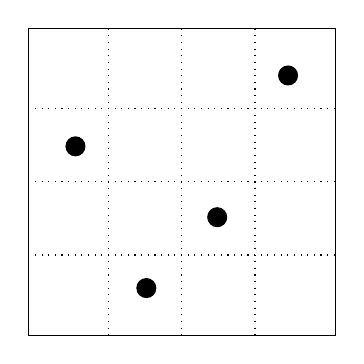
\begin{tikzpicture}[scale=.3]
        \draw[black] (0,0) -- (13,0) -- (13,13) -- (0,13) -- cycle;
        \draw[fill=black] (2,8) circle (4mm);
        \draw[fill=black] (5,2) circle (4mm);
        \draw[fill=black] (8,5) circle (4mm);
        \draw[fill=black] (11,11) circle (4mm);
        \foreach \i in {3.4, 6.5, 9.6}{
          \draw[dotted] (0,\i) -- (13,\i);
          \draw[dotted] (\i,0) -- (\i,13);
        }
      \end{tikzpicture}
      \hspace{1pc}
      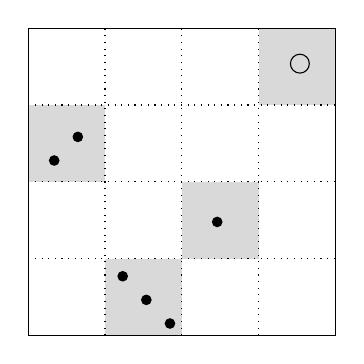
\begin{tikzpicture}[scale=.3]

        \draw[draw=none,fill=black!15] (0, 6.5) rectangle (3.25,9.75);
        \draw[draw=none,fill=black!15] (3.25, 0) rectangle (6.5,3.25);
        \draw[draw=none,fill=black!15] (6.5, 3.25) rectangle (9.75,6.5);
        \draw[draw=none,fill=black!15] (9.75, 9.75) rectangle (13,13);

        \draw[black] (0,0) -- (13,0) -- (13,13) -- (0,13) -- cycle;

        \foreach \i in {3.25, 6.5, 9.75}{
          \draw[dotted] (0,\i) -- (13,\i);
          \draw[dotted] (\i,0) -- (\i,13);
        }


        \draw[fill = black] (1.1,7.4) circle (2mm);
        \draw[fill = black] (2.1,8.4) circle (2mm);

        \draw[fill = black] (4, 2.5) circle (2mm);
        \draw[fill = black] (5, 1.5) circle (2mm);
        \draw[fill = black] (6, .5) circle  (2mm);

        \draw[fill = black] (8,4.8) circle (2mm);

        \draw[] (11.5,11.5) circle (4mm);
      \end{tikzpicture}
      \hspace{1pc}
      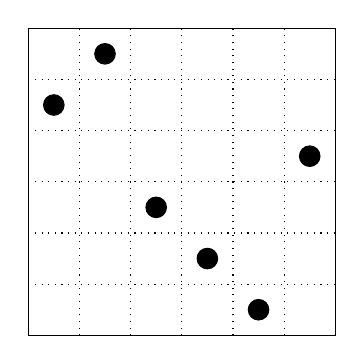
\begin{tikzpicture}[scale=.325]
        \draw[black] (0,0) -- (12,0) -- (12,12) -- (0,12) -- cycle;
        \draw[fill = black] (1,9) circle (4mm);
        \draw[fill = black] (3,11) circle (4mm);

        \draw[fill = black] (5,5) circle (4mm);
        \draw[fill = black] (7,3) circle (4mm);
        \draw[fill = black] (9,1) circle (4mm);

        \draw[fill = black] (11,7) circle (4mm);

        \foreach \i in {2,4,6,8,10} {
          \draw[dotted] (\i, 0) -- (\i, 12);
          \draw[dotted] (0,\i) -- (12,\i);
        }
      \end{tikzpicture}
    \caption{The peg permutation $\tro = \pl3 \mn1 \dt2 \pl4$ inflated by the
    vector $\vec{i} = (2,3,1,0)$ is the permutation $563214$.}
    \label{polyclass:fig:inflation}
    \end{figure}
    
    \begin{definition} \label{polyclass:def:inflations}
      For a peg permutation $\tro$, denote by $\I(\tro)$ the set of all valid
      inflations of $\tro$. Similarly, for a set $\tS$ of peg permutations, let 
      $$ \I(\tS) = \cup_{\tro \in \tS} \I(\tro).$$
      It follows that for a permutation $\pi \in \I(\tro)$, there exists some
      partition $P$ of the entries of $\pi$ into monotone intervals which are
      compatible with $\tro$. This partition is referred to as a
      $\tro$-partition of $\pi$. 
    \end{definition}

    It can be easily shown that, for a peg permutation $\tro$ of length $n$, if
    $\vec v = (v_1, v_2 \dots v_n) \in \Zgeq^n$ and $\vec w = (w_1, w_2, \dots
    w_n) \in \Zgeq^n$ are two vectors such that $v_i \leq w_i$ for all $i \in [n]$,
    then $\tro(\vec v) \prec \tro(\vec w)$ as permutations. Also, note that
    $\I(\tro)$ forms a permutation class, and in fact, as we shall soon see, a
    polynomial class. 

    \begin{theorem}[\cite{SophieVince, GridClasses}] \label{polyclass:thm:tfae}
      For a permutation class $\C$, the following are equivalent. 
      \begin{enumerate}[1)]
        \item $\C$ is a polynomial class,
        \item $\C_n < f_n$ for some $n$, where $f_n$ is the $n$th Fibonacci
        number,
        \item $\C$ does not contain arbitrarily long patterns of the forms
        shown in Figure~\ref{polyclass:fig:alternations},
        \item $\C = \I(\tS)$ for some set $\tS$ of peg permutations. 
      \end{enumerate}
    \end{theorem}

    \begin{figure}[t] \centering
      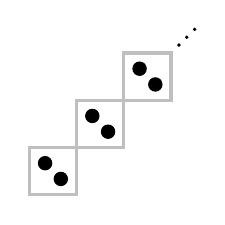
\begin{tikzpicture}[scale=.2]

        % loops over the 3 boxes
        \foreach \i in {1, 4, 7}{
          \draw[very thick, color=lightgray] 
          (\i,\i) -- (\i, \i+3) -- (\i+3, \i+3) -- (\i+3,\i) -- cycle;
          \draw[fill = black] (\i+2, \i+1) circle (12pt);
          \draw[fill = black] (\i+1, \i+2) circle (12pt);
          }

        % had to draw the ellipses by hand...
        \draw[fill = black] 
              (10.5,10.5) circle (2pt)
              (11,11) circle (2pt)
              (11.5,11.5) circle (2pt);
      \end{tikzpicture}
        \hspace{2em}
      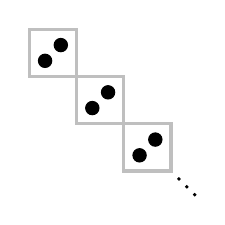
\begin{tikzpicture}[scale=.2]
        \foreach \i in {1, 4, 7}{
          \draw[very thick, color=lightgray] 
          (\i,12-\i) -- (\i, 12-\i-3) -- (\i+3,12-\i-3) -- (\i+3,12-\i) -- cycle;
          \draw[fill = black] (\i+2, 12-\i-1) circle (12pt);
          \draw[fill = black] (\i+1, 12-\i-2) circle (12pt);
          }

        \draw[fill = black] 
              (10.5,1.5) circle (2pt)
              (11,1) circle (2pt)
              (11.5,0.5) circle (2pt);
      \end{tikzpicture}
        \hspace{2em}
      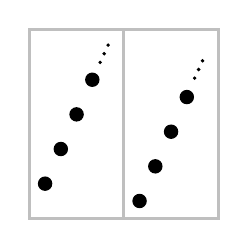
\begin{tikzpicture}[scale = .2]
        % draws the boundaries
        \draw[very thick, color = lightgray]
          (6,0) -- (6,12) -- (12,12) -- (12,0) -- (0,0) -- (0,12) -- (6,12);

        % draws the permutation
        \foreach \y [count = \x] in {2,4,6,8}
          \draw[fill = black] (\x, 1.1*\y) circle (12pt);
        \foreach \y [count = \x] in {1,3,5,7}
          \draw[fill = black] (\x + 6, 1.1*\y) circle (12pt);

        % draws dots
        \foreach \x/\y in {4.5/9, 4.75/9.5, 5/10}
        \draw[fill = black]
          (\x, 1.1*\y) circle (2pt);

        \foreach \x/\y in {4.5/9, 4.75/9.5, 5/10}
        \draw[fill = black]
          (\x + 6, 1.1*\y - 1) circle (2pt);
      \end{tikzpicture}
        \hspace{2em}
      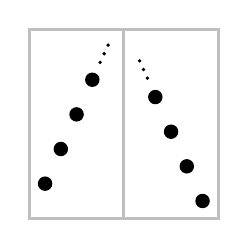
\begin{tikzpicture}[scale = .2]
        % draws the boundaries
        \draw[very thick, color = lightgray]
          (6,0) -- (6,12) -- (12,12) -- (12,0) -- (0,0) -- (0,12) -- (6,12);

        % draws the permutation
        \foreach \y [count = \x] in {2,4,6,8}
          \draw[fill = black] (\x, 1.1*\y) circle (12pt);
        \foreach \y [count = \x] in {1,3,5,7}
          \draw[fill = black] (12-\x, 1.1*\y) circle (12pt);

        % draws dots
        \foreach \x/\y in {4.5/9, 4.75/9.5, 5/10}
        \draw[fill = black]
          (\x, 1.1*\y) circle (2pt);

        \foreach \x/\y in {4.5/9, 4.75/9.5, 5/10}
        \draw[fill = black]
          (12- \x, 1.1*\y - 1) circle (2pt);
      \end{tikzpicture}

    \caption{If a class contains arbitrarily long patterns of any of these forms,
    it is not a polynomial class.}
    \label{polyclass:fig:alternations}
    \end{figure}


  \subsection{Peg Patterns}

    Analogous to the permutation pattern ordering, we can define an ordering on
    peg permutations. Essentially, we say that a peg permutation is contained in
    another if it can be obtained by deleting entries and changing signs to dots. 


    \begin{definition} \label{polyclass:def:pegpattern}
      Let $\tro = \tro_1 \tro_2 \dots \tro_n$ and $\ttau = \ttau_1 \ttau_2 \dots
      \ttau_k$ be peg permutations. Say that $\ttau$ is contained within $\tro$ if
      there is a subsequence $\tro_{i_1} \tro_{i_2} \dots \tro_{i_k}$, whose
      entries lie in the same relative order as those of $\ttau$ and whose
      decorations are \emph{compatible}, meaning that $\tro_{i_j}$ either have
      the same decoration or $\ttau_j$ is decorated with a dot. 
    \end{definition}

    It follows from the definitions that if $\ttau \prec \tro$, then $\I(\ttau)
    \subset \I(\tro)$. However, the converse is not true. For example, letting
    $\ttau = \dt 1 \dt 2$ and $\tro = \pl 1$, we see that $\I(\ttau) = \{1, 12\}
    \subset \I(\tro)$, but $\ttau \not \prec \tro$. The core idea of the algorithm
    is the partition all permutations of the class according to peg permutation,
    and then enumerate these by enumerating integer vectors. 

    \begin{definition} \label{polyclass:def:fillingperm}
      For a peg permutation $\tro$ and a permutation $\pi$, say that $\pi$
      \emph{fills} $\tro$ if $\pi = \tro(\vec v)$ such that $\vec v_i = 1$
      whenever $\tro_i$ is decorated with a dot, and $\vec v_i \geq 2$
      otherwise. Every peg permutation $\tro$ has a unique minimal filling
      permutation, denoted $m_{\tro}$. 
    \end{definition}

    



  \subsection{Integer Vectors}

    Peg permutations provide a way of translating between integer vectors and
    permutations. The underlying idea of the algorithm is to formalize this
    correspondence in a way which preserves the ordering, converting permutation
    posets into posets of integer vectors. We will now establish some machinery
    for working with and enumerating integer vector posets.

    Downsets in the integer vector poset are easier to work with than permutation
    classes in part because of Higman's Theorem~\cite{HigmansThm}, which
    implies that every downset has a finite basis. The union and intersection
    of these downsets is easy to compute as well. 

    \begin{definition} \label{polyclass:def:vecposet}
      For two vectors $\vec v, \vec w \in \Zgeq^n$, say that $\vec v \prec \vec
      w$ if $v_i \leq w_i$ for each $i \in [n]$.  For a downset $\cV \subset
      \Zgeq^n$, denote by $\cB_\cV$ the set of minimal vectors in the
      complement of $\cV$. It follows then that $\cV$ can be described as
      precisely those vectors which \emph{avoid} the vectors of $\cBV$, that
      is, 

      $$ \cV := \{ \vec v \in \Zgeq^n : \vec b_i \not \prec \vec v, \frall
          \vec b_i \in \cBV \}. $$

      For two vectors $\vec v, \vec w \in \Zgeq^n$, denote by $\vec v \vee \vec
      w$ the minimal vector for which $\vec v \prec \vec v \vee \vec w$ and $\vec
      w \prec \vec v \vee \vec w$. It follows that $ (\vec v \vee \vec w)_i =
      \max(\vec v_i, \vec w_i)$ for each $i \in [n]$. 
    \end{definition}


    \begin{proposition} \label{polyclass:prop:vectorunions}
      Let $\cV, \cW$ be downsets in $\Zgeq^n$ with corresponding downsets $\cBV,
      \cBW$.  Letting $\cBM$ be the minimal vectors of the set $\{\vec v \vee
      \vec w : \vec v \in \cV, \vec w \in \cW \}$, 
      $\cBU$ the minimal vectors of the union $\cBV \cup \cBW$, and $\cM$
      and $\cU$ the downsets which avoid $\cBM$ and $\cBU$, respectively. We
      have that 
      $$ \cV \cap \cW = \cU, $$
      $$ \cV \cup \cW = \cM .$$
    \end{proposition}
    \begin{proof}
      Clearly, any vector in $\cV \cap \cW$ must avoid all basis elements of
      both $\cBV$ and $\cBW$, and so the basis for $\cV \cap \cW $ is the set
      of minimal elements of the set $\cBV \cup \cBW$. For
      unions, we proceed using De Morgan's laws:
      $$ \begin{aligned}
        \cV \cup \cW
        &= \left( \bigcap_{\vec v \in \cBV} \{\vec v \mbox{-avoiding
              vectors}\}\right) \bigcup
           \left( \bigcap_{\vec w \in \cBW} \{\vec w \mbox{-avoiding
              vectors}\}\right) \\
        &= \bigcap_{\substack{ \vec v \in \cBV \\ \vec w \in \cBW }} 
          \Big( \{\vec v \mbox{-avoiding vectors}\} 
            \cup \{\vec w \mbox{-avoiding vectors}\}\Big) \\
        &= \bigcap_{\substack{ \vec v \in cBV \\ \vec w \in \cBW }} 
            \{\vec v \vee \vec w \mbox{-avoiding vectors}\}.
        \end{aligned} $$

      Therefore the basis for $\cV \cup \cW$ consists of the set $\cBM$,
      completing the proof.
      \end{proof}

      Proposition~\ref{polyclass:prop:vectorunions} can also be used to enumerate 
      downsets of integer vector classes, using inclusion exclusion. It will be
      useful to consider these downsets as collections of point-sets on an integer
      lattice, and to enumerate the classes based on the number of $n$-element
      sets they contain. We formalize this below. 

    We define the \emph{weight} of a vector as the sum of its entries. A peg
    permutation, inflated by a vector of weight $k$, produces a permutation of
    length $k$. Counting integer vectors according to weight is relatively
    simple, and is equivalent to counting ordered compositions. Letting
    $a_{n,k}$ denote the number of $k$-weight vectors in $\Zgeq^n$, we have 
    $$ \sum_{k \geq 0} a_{n,k} z^k = \frac{1}{(1 - z)^n}.$$

    Similarly, the generating function for the number of permutations which
    contain a given vector $\vec v \in \Zgeq^n$ is given by 
    $$ \frac{z^{\wt(\vec v)}}{(1 - z)^n} .$$
    It follows from this and Proposition~\ref{polyclass:prop:vectorunions} that
    that downsets can be enumerated by adding and subtracting generating
    functions of this form. This leads to the following lemma. 

    \begin{lemma} \label{polyclass:lem:fillinggfcn}
      Let $\tro$ be a peg permutation, and let $s$ be the number of signs in
      the decoration of $\tro$, and $d$ the number of dots. Then the generating
      function for the filling permutations of $\tro$ is given by 
      $$ \frac{z^{d + 2s}}{(1 - z)^s}.$$ 
    \end{lemma}
    
    Lemma~\ref{polyclass:lem:fillinggfcn} will ultimately be our enumeration
    scheme for these classes. The main barrier is partitioning the class
    into categories based on which peg permutation they fill. The bulk of the
    algorithm, described in the next section, will be performing this
    partitioning. 
        

% =========================================================================== %
\section{The Algorithm}
\label{polyclass:sec:algo}
% =========================================================================== %

  This section gives an overview of the enumeration algorithm, given a set of
  peg permutations as an input, and outputting a disjoint set of integer vector
  downsets, which can then be enumerated. The algorithm consists of three
  parts. First the set is \emph{completed}, then \emph{compacted}, and finally
  \emph{cleaned}, at which point we have a set of peg permutations which
  partition the class. Letting $\tS$ be a set of peg permutations, we describe
  each part in detail below, with the goal of enumerating the class $\I(\tS)$.
  A pseudocode overview of the algorithm is shown in
  Figure~\ref{polyclass:fig:pseudocode}.

  \subsection{Completing the Set}
    Say that a set $\tS$ is \emph{complete} if every permutation $\pi \in
    \I(\tS)$ fills at least one element $\tro \in \tS$. For example, the set
    $\{\pl 2 \pl 1\}$ is not complete, because $1\ 2\ 3 \in \I(\pl 2 \pl 1)$
    (since $1\ 2\ 3 = \pl 2 \pl1 (3,0)$), but doesn't fill $\pl 2 \pl 1$. It
    follows from the definition of peg patterns, however, that every
    permutation in $\I(\tS)$ must fill some pattern within an element in $\tS$. 

    Therefore, the downset of any peg pattern is a complete set.  The first
    step of the algorithm completes the set $\tS$ by, 
    for each $\tro \in \tS$, we add all patterns of $\tro$ into the set $\tS$.
    After this step, the set $\tS$ is complete. 

  \subsection{Compacting the Set}


    The next obstacle in the enumeration is ensuring that every permutation in
    the class fills a unique peg permutation in the set.  Given a permutation,
    we can divide its entries up into monotone intervals in a number of ways.
    The following lemma will help to ensure uniqueness, and allow for
    enumeration. 

    \begin{lemma} \label{polyclass:lem:intervals}
      If two monotone intervals intersect, then their union and intersection
      are also monotone intervals.
    \end{lemma}
    \begin{proof}
      Suppose we have two monotone intervals with a non-empty intersection.
      Without loss of generality, suppose that one of them is increasing, and
      so their intersection is either increasing or consists of a single
      element. Since each interval consists of contiguous entries, the second
      entry must also be increasing, and so the union of the two is an
      increasing interval. 
    \end{proof}
    
    Lemma~\ref{polyclass:lem:intervals} implies that by greedily choosing the
    largest possible intervals, we can ensure that for each permutation $\pi$,
    there is a unique smallest peg permutation $\tro$ for which $\pi$ is in
    $\I(\tro)$, but not in $\I(\ttau)$ for any $\ttau \prec \tro$. However, not
    all peg permutations are able to fulfill this role. 

    Say that a peg permutation $\tro$ is \emph{compact} if, for all $\ttau \prec
    \tro$, we have that $\I(\ttau) \not = \I(\tro)$. For example, $\dt 2 \mn 1$
    is not compact, since $\I(\dt 2 \mn 1) = \I(\mn 1)$. The following
    lemma and proposition characterizes these peg permutations. 



    \begin{proposition}\label{polyclass:prop:compact}
      For a peg permutation $\tro$, the following are equivalent:
      \begin{enumerate}[1)]
      \item $\tro$ is compact, 
      \item $\tro$ does not contain the patterns $\pl1 \pl2, \pl1 \dt2, \dt1
        \pl2$ or, symmetrically, $\mn2 \mn1, \mn2 \dt1$ or $\dt2 \mn 1$, 
      \item every permutation $\pi$ which fills $\tro$ has a unique vector
        $\vec v$ for which $\tro(\vec v) = \pi$. 
      \end{enumerate}
    \end{proposition}
    \begin{proof}
      First we show that (1) and (2) are equivalent. Clearly (1) implies (2),
      so to show the reverse implication, let $\tro$ be a noncompact peg
      permutation. By definition, there exists some $\ttau \prec \tro$ such that
      $\I(\ttau) = \I(\tro)$. Let $\pi$ be a permutation which fills $\tro$,
      with $P$ the $\tro$-partition and $P'$ the $\ttau$ partition. Because
      $\ttau$ is shorter than $\tro$, it follows that there must be some part
      of $P'$ which intersects two parts of $P'$. By
      Lemma~\ref{polyclass:lem:intervals} these two form a monotone
      interval, and so must be of one of the forms listed in (2). 

      Now, we show that (2) and (3) are equivalent. If a peg permutation
      $\tro$ contains one of the patterns specifies in (2), it is clear that a
      permutation can fill $\tro$ in at least two different ways, so (3)
      implies (2). Suppose that the permutation $\pi$ fills $\tro$ with two
      different $\tro$-partitions $P$ and $P'$. It follows then that
      a block of one partition must intersect two blocks of the other. However,
      this implies (Lemma~\ref{polyclass:lem:intervals}) that intersection
      and unions are also monotone, and so must be of one of the forms given in
      (2). 
    \end{proof}

    By simply removing each of the peg permutations which contain one of the
    intervals listed in Proposition~\ref{polyclass:prop:compact}, our set of
    peg permutations becomes a set of compact peg permutations. Further, since
    our set is a full and complete downset, the definition of compact implies
    that the new set will still be complete. 

  \subsection{Cleaning the Set}

    The final step in the algorithm is bijecting our complete and compact set
    of peg permutations to a set of downsets of integer vectors. Our final
    obstacle in this bijection will be peg permutations which have intervals of
    dotted entries. For example, the peg permutation $\dt 1 \dt 2 \dt 3 \dt 4$
    produces a class which is strictly contained in $\pl 1$, but there is no
    containment at the level of peg permutations. We remedy this by using
    forbidden vectors: the peg permutation $\dt 1 \dt2 \dt 3 \dt4$ is mapped to
    the inflations of $\pl 1$ which \emph{avoid} the vector $\vect{5}$. 

    \begin{definition} \label{polyclass:def:clean}
      Say that a peg permutation $\tro$ is \emph{clean} if $\I(\tro) \not
      \subset \I(\ttau)$ for any shorter permutation $\ttau$. 
    \end{definition}

    \begin{proposition}\label{polyclass:prop:clean}
      The compact peg permutation $\tro$ is clean if and only if it does not
      contain an interval order isomorphic to $\dt 1 \dt 2$ or $\dt 2 \dt 1$. 
    \end{proposition}
    \begin{proof}
      If $\tro$ contains one of the specified intervals, then letting $\ttau$ be
      the shorter peg permutation obtained by contracting these two entries
      into a single entry with the appropriate sign, we find that $\I(\tro)
      \subseteq \I(\ttau)$. 

      For the other direction, suppose that $\I(\tro) \subseteq \I(\ttau)$ for
      some shorter peg permutation $\ttau$. Let $\pi$ be any permutation which
      fills $\tro$. In any $\ttau$-partition of $\pi$ there must be a monotone
      interval formed from entries in different parts of any $\tro$ partition.
      Because $\tro$ is compact, it follows (from
      Proposition~\ref{polyclass:prop:compact}) that $\tro$ must contain either
      $\dt 1 \dt 2$ or $\dt 2 \dt 1$, completing the proof.
    \end{proof}

    Given a complete and compact set $\tS$ of peg permutations, it is not
    possible in general to find a clean set which inflates to the same class.
    To see this, let $\tro = \dt 1 \dt 2 \dt 3$. Then there is no clean set
    whose inflation is equal to $\I(\tro)$. However, we can put the set $\tS$
    in bijection with a clean set \emph{together} with a set of allowable
    inflation vectors. We formalize this below. 

    \begin{definition}\label{polyclass:def:restricted-inflations}
      For a peg permutation $\tro$ and a set $\cV$ of vectors of the same
      length, let $\I(\tro;\cV)$ denote the inflations of $\tro$ using vectors
      from the set $\cV$. 
    \end{definition}

    \begin{lemma}\label{polyclass:lem:clean}
      For each peg permutation $\tro$, there exists a clean permutation $\ttau$
      and a vector set $\cV$ such that the set of all inflations of $\tro$ is equal
      to $\I(\ttau, \cV)$. 
    \end{lemma}
    \begin{proof}
      To construct $\ttau$, simply contract all of the intervals of dotted
      entries in $\tro$ into signed entries. To construct $\cV$, build a vector
      $\vec v$ such that, if the entry $\ttau_i$ arose from a dotted interval
      of length $k$, let $\vec v_i = k+1$, and take $\cV$ to be the set of
      vectors avoiding $\vec v$.  This ensures that this entry will never be
      inflated by a run longer than the original sequence of dotted entries.
    \end{proof}

    The final step of the algorithm can be described as follows. First, let $\fV$ be
    an empty set, which will be the output. For each peg permutation $\tro \in \tS$, 
    compute the pair $(\ttau, \vec W)$ as described in
    Lemma~\ref{polyclass:lem:clean}, and let $\cV$ be the vector downset with
    basis $\cBV = \{\vec v\}$. 
    If there is no pair $(\ttau, \cW)$ in the
    set $\fV$, add $(\ttau, \cV)$ to $\fV$. 
    Otherwise, replace $(\ttau, \cW)$ with $(\ttau, \cW \cup \cV)$. 

    Since every permutation in the class fills a unique clean and compact
    peg permutation, and since each permutation which fills a compact
    permutation has a unique partition, it follows that the polynomial class is
    in bijection with the set 
    $$ \biguplus_{(\tro,\cV) \in \fV} \I(\tro, \cV).$$

    Letting $\vec m_{\tro}$ be the vector defined by $(\vec m_{\tro})_i
    = 1$ if $\tro_i$ is decorated with a dot, and $(\vec m_{\tro})_i = 2$
    otherwise, and let $s(\tro)$ denote the number of signed (non-dotted)
    entries of $\tro$. The generating function for $\I(\tro)$ is then given by
    inclusion exclusion in conjunction with
    Proposition~\ref{polyclass:prop:vectorunions}, and allows us to efficiently
    enumerate these classes.  
    $$ \sum_{B \subseteq \cBV} (-1)^{|B|} 
        \frac{ z^{\wt \left( \vec m_{\tro} \vee (\bigvee B)\right)}}{%
        {(1-z)}^{ s( \tro ) } }.  $$



  \SetAlFnt{\small\ttfamily}
  \begin{algorithm}
    \DontPrintSemicolon
    \KwIn{Set $\tS$ of Peg Permutations}
    \KwOut{Integer vectors in bijection with the class}

    \tcp{Complete $\tS$}
    \For{$\tro \ \in \tS$}{
      Add to $\tS$ all peg permutations which can be realized by deleting entries of
      $\tro$, or changing a signs to dots\;
    }

    \tcp{Remove all non-compact elements from $\tS$}
    \For{$\tro\ \in \tS$}{
      \If{\ttfamily $\tro$ contains any of the consecutive permutations 
      $\pl{1}\pl{2}, \dt{1}\pl{2}, \pl{1}\dt{2}$ or their symmetries
      }{ 
      Remove $\tro$ from $\tS$\; }
    }

    \tcp{Clean $\tS$ and construct a vector set}
    Initialize the set $\mathfrak{V}$, which will contain pairs $(\tro,
    \cV)$, where $\tro$ is a peg permutation and $\cV$ is a set of
    integer vectors of the same length as $\tro$\;
    \For{$\tro \  \in $ $\tS$}{
      \eIf{\ttfamily $\tro$ contains intervals of the form $\dt{1}\dt{2}$ or
      $\dt{2}\dt{1}$}
      { Let $\ttau$ denote the cleaned $\tro$, and $\cV$ the set of integer
      vectors for which $\{\ttau[\vec{v}] : \vec{v} \in \cV\}  = \{\tro[\vec{v}]
      : \vec{v} \in \mathcal{F}_{\tro}\} $\; Let $(\tro',\cV')
      \leftarrow (\ttau, \cV)$\;
      }
      { 
        Let $(\tro', \cV') \leftarrow  (\tro, \mathcal{F}_{\tro})$\;
      }
      \eIf{\ttfamily $(\tro', \cW) \in \mathfrak{V}$ for some $\cW$}{
        Replace the element $(\tro',\cW)$ with $(\tro', \cW \cup \cV')$\;
      }
      {
        Add $(\tro', \cV')$ to $\mathfrak{V}$\;
      }
    }
    The permutation class is now in bijection with the disjoint union
    $\displaystyle\biguplus_{(\tro,\cV) \in \mathfrak{V}} \{
      \tro[\vec{v}] : \vec{v} \in \cV \}$.\; 
  \SetAlFnt{\normalsize\sffamily}
  \caption{A pseudocode overview of the algorithm.}
  \label{polyclass:fig:pseudocode}
  \end{algorithm}



% =========================================================================== %
\section{Genomics}
\label{polyclass:sec:data}
% =========================================================================== %

  The field of computational biology is a new and rapidly developing field.
  The vast quantities of sequencing data produced by modern geneticists
  necessitate the use of complex mathematical techniques for analysis.
  A common problem, given two related genetic sequences, is to determine the
  most recent evolutionary ancestor. This is generally solved by determining
  the number of mutations required to rearrange one sequence into the other,
  allowing a researcher to determine the midpoint between the two. Determining
  this distance, however, is computationally difficult, but the work presented
  in this chapter can be used to effectively and efficiently perform these and
  other computations. 
  
  This section applies the theory of polynomial classes to the problem of
  evolutionary distance. 
  While the focus is on the combinatorial aspects of genome
  rearrangement, we begin with a rough overview of the biological mechanics.
  For a more complete introduction, see the surveys \cite{CompBio} or
  \cite{GenomeBook}.
  

  \subsection{Chromosomes and Mutation}
      
    Every living organism encodes its hereditary information in molecules
    called \emph{chromosomes}, the set of which is known as the organism's
    \emph{genome}. The information carried in the genome is passed down from
    organism to organism, and undergoes mutations which can cause both subtle
    and dramatic change between generations. 
  
    Each chromosome is composed of double strands of deoxyribonucleic acid
    (DNA), each strand of which is in turn composed of a sequence of
    \emph{nucleotides}. Nucleotides come in four types (A, C, G, and T), and
    the two strands, arranged in a double helix, are complementary, i.e., a A's
    are always coupled with a T, and G's with C. It follows that DNA can be
    defined as a single sequence - a \emph{word} on the alphabet
    $\{\text{A,C,G,T}\}$. A DNA \emph{sequence} is some consecutive piece of
    this word, while \emph{genes} are the smallest sequences which have some
    independent biological function.
    
    The genome is made up of chromosomes, which are in turn made up of coiled
    DNA strands, which can be broken down into genes sequences, which
    themselves are simply sequences of nucleotides. This complexity leads to
    a variety of errors which can be introduced during replication, and these
    inaccuracies are the basis for genetic evolution. Many of these
    mutations can be viewed as rearranging sequences of genes, and can be
    effectively modelled using permutations. 

    The physical properties of chromosomes lead to a variety of rearrangement
    operations, but they share a common theme: some contiguous segment of the
    gene sequence is removed, reversed and/or relocated, then replaced back in
    the sequence. While there are other mutations possible at both the larger
    and smaller scales, these so called \emph{genome-rearrangements} have
    received much attention in recent research and, most importantly, fall
    under the purview of polynomial classes.



  \subsection{Block Transformations}
  
    Permutations are apt models for rearrangement, and can be used to study
    genetic mutations. Mutations happen in various ways, and a variety of
    permutation transformations have been studied. These operations are known
    collectively as \emph{block transformations}, as each of them acts on
    contiguous subsequences of permutations, henceforth referred to as
    \emph{blocks}. Each of these operations can be viewed as a set of allowable
    moves which transform one permutation into another. 
    
    Treating block transformations as mutations, the basic problem is as
    follows: given two permutations, what is the shortest sequence of moves
    which can transform one into the other? By relabelling the entries, we can
    assume, without any loss of generality, that the target permutation is the
    identity permutation. In this light, the question becomes a \emph{sorting}
    sorting problem, and asks how quickly a sequence can be sorted.  We present
    here some of the more commonly studied operations, but note that other
    varieties and models are biologically significant.  

    \begin{definition} \label{polyclass:def:block}
      Let $\pi = \pi_1 \pi_2 \dots \pi_n$ be a permutation written in one-line
      notation. A \emph{block} of $\pi$ is some contiguous string of entries 
      $\pi_{i} \pi_{i + 1} \dots \pi_{i+k}$. 
      A \emph{prefix} is a block which starts at $\pi_1$. 
    \end{definition}

    Blocks of permutations are models for gene sequences, and each of the block
    permutations below differ only in their treatment of blocks. We define each
    type of sorting by defining a single allowable operation. 

    \begin{definition}[Block Reversal]\label{polyclass:def:blockrev}
      A \emph{block reversal} operation consists of reversing the entries of
      any block of the permutation. This operation was first studied by
      Watterson, Ewens, Hall, and Morgan~\cite{Watterson1982} and further
      investigated by Alpar-Vajk~\cite{Alpar2009}.
    \end{definition}
    
    \begin{definition}[Block Transposition]\label{polyclass:def:blocktrans}
      A \emph{block transposition} operation consists of moving one block
      from its current position to any other location in the permutation. 
      This operation was first studied by Bafna and Pevzner~\cite{Bafna1998}. 
    \end{definition}
  
    \begin{definition}[Block Interchange]\label{polyclass:def:blockint}
      A \emph{block interchange} operation consists of selecting two
      non-intersecting blocks of the permutation and interchanging them. 
      This operation was first studied by Christie~\cite{Christie1996}, and
      further investigated by B\'ona and Flynn~\cite{Bona2009}. 
    \end{definition}
  
    \begin{definition}[Prefix Transposition]\label{polyclass:def:prefixtrans}
      A \emph{prefix transposition} operation consists of moving a prefix of
      the permutation to any other location in the permutation. 
      This operation was first studied by Dias and Meidanis~\cite{Dias2002}.
    \end{definition}
      
    \begin{definition}[Prefix Reversal]\label{polyclass:def:prefixrev}
      A \emph{prefix reversal} operation consists of reversing the entries of a
      prefix of the permutation. This is sometimes referred to as the `pancake
      flipping operation', and was first studied by ``Harry Dweighter''
      (actually, Jacob E. Goodman) as a \emph{Monthly}
      problem~\cite{Dweighter} (and was also studied by Gates~\cite{BillGates}). 
    \end{definition}
  
    \begin{definition}[Cut-Paste Sorting]\label{polyclass:def:cutpaste}
      A \emph{cut-paste} operation consists of moving a block of the
      permutation, with the option to reverse its entries. 
      This operation was first studied by Cranston, Sudborough, and
      West~\cite{Cranston2007}. 
    \end{definition}
  
    For a given block transformation, we refer to the \emph{distance} between
    two permutations $\pi$ and $\sg$ as the minimum number of operations needed
    to transform one into the other. Finding the maximal distance between two
    permutations of a given length is equivalent to finding the maximal
    distance from the identity to any permutation. Further, since each of these
    operations is reversible --- if $\pi$ can be transformed into $\sg$, then
    $\sg$ can be transformed into $\pi$ --- this is equivalent to finding the
    distance from the identity to any permutation. 


    Biologically, two permutations with a small distance represent closely
    related organisms, as each transformation represents a mutation which can
    occur from one generation to the next. Understanding the sets of
    permutations at each fixed distance from the identity can help to
    understand how different genomes are related. For any $k \in \Zgeq$, the
    set of permutations which are at distance $\leq k$ from the identity forms
    a polynomial class, and thus can be enumerated by our algorithm. 

    \begin{theorem} \label{polyclass:def:operation-polyclass}
      For each of the operations presented above and for a positive integer
      $k$, the set of permutations with distance at most $k$ from the identity
      forms a polynomial class. 
    \end{theorem}
    \begin{proof}
      The class of identity permutations is the inflations of the peg
      permutation $\pl 1$, which can be represented geometrically as a diagonal
      line parallel to $y =x $. Each block transformation can be viewed as
      taking some piece of this line and moving or reversing it. Such an array
      of lines can be translated back into a peg permutation, and it follows
      that the set of distance $\leq k$ permutation can be represented as the
      union of all peg permutations obtained in this way.  See
      Figures~\ref{polyclass:fig:blockrev} and~\ref{polyclass:fig:twoblockrevs}
      for graphical examples. 
    \end{proof}


    \begin{figure}[t] \centering
      \begin{tikzpicture}[scale=.3]
        \draw[black] (0,0) -- (12,0) -- (12,12) -- (0,12) -- cycle;
        \foreach \i in {4,8}{
          \draw[dotted] (0, \i) -- (12, \i);
          \draw[dotted] (\i, 0) -- (\i, 12);
        }
        \draw (0,0) -- (4,4);
        \draw (4,8) -- (8,4);
        \draw (8,8) -- (12,12);
      \end{tikzpicture}
      \hspace{1pc}
      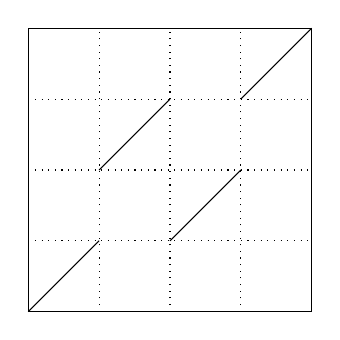
\begin{tikzpicture}[scale=.3]
        \draw[black] (0,0) -- (12,0) -- (12,12) -- (0,12) -- cycle;
        \foreach \i in {3,6,9}{
          \draw[dotted] (0, \i) -- (12, \i);
          \draw[dotted] (\i, 0) -- (\i, 12);
        }
        \draw (0,0) -- (3,3);
        \draw (3,6) -- (6,9);
        \draw (6,3) -- (9,6);
        \draw (9,9) -- (12,12);
      \end{tikzpicture}
      \hspace{1pc}
      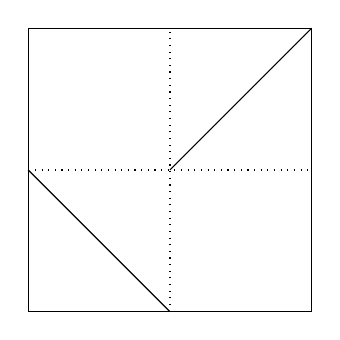
\begin{tikzpicture}[scale=.3]
        \draw[black] (0,0) -- (12,0) -- (12,12) -- (0,12) -- cycle;
        \foreach \i in {6}{
          \draw[dotted] (0, \i) -- (12, \i);
          \draw[dotted] (\i, 0) -- (\i, 12);
        }
        \draw (0,6) -- (6,0);
        \draw (6,6) -- (12,12);

      \end{tikzpicture}
      \caption[The classes of permutations which are at most one block 
      reversal]{The classes of permutations which are at most one block
      reversal, block transposition, and prefix reversal away from the identity
      are given by $\I(\pl 1 \mn 2 \pl 3)$, $\I(\pl 1 \pl 3 \pl 2 \pl 4)$, and 
      $\I(\mn 1 \pl 2)$, respectively.}
      \label{polyclass:fig:blockrev}
    \end{figure}


    \begin{figure}[t] \centering
      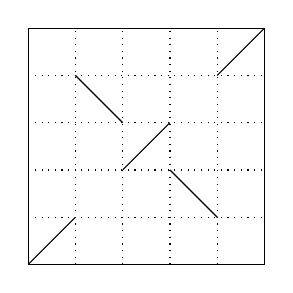
\begin{tikzpicture}[scale=.2]
        \draw[black] (0,0) -- (15,0) -- (15,15) -- (0,15) -- cycle;
        \foreach \i in {3,6,9,12}{
          \draw[dotted] (0, \i) -- (15, \i);
          \draw[dotted] (\i, 0) -- (\i, 15);
        }
        \draw (0,0) -- (3,3);
        \draw (12,12) -- (15,15);
        \draw (3, 12) -- (6,9);
        \draw (6,6) -- (9,9);
        \draw (9,6) -- (12,3);

      \end{tikzpicture}
      \hspace{4pt}
      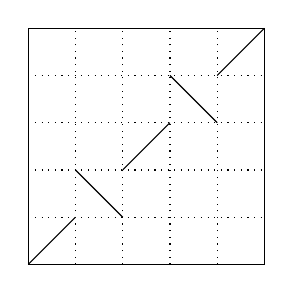
\begin{tikzpicture}[scale=.2]
        \draw[black] (0,0) -- (15,0) -- (15,15) -- (0,15) -- cycle;
        \foreach \i in {3,6,9,12}{
          \draw[dotted] (0, \i) -- (15, \i);
          \draw[dotted] (\i, 0) -- (\i, 15);
        }
        \draw (0,0) -- (3,3);
        \draw (12,12) -- (15,15);
        \draw (3, 6) -- (6,3);
        \draw (6,6) -- (9,9);
        \draw (9,12) -- (12,9);

      \end{tikzpicture}
      \hspace{4pt}
      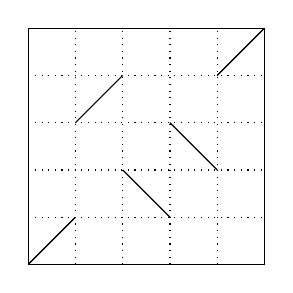
\begin{tikzpicture}[scale=.2]
        \draw[black] (0,0) -- (15,0) -- (15,15) -- (0,15) -- cycle;
        \foreach \i in {3,6,9,12}{
          \draw[dotted] (0, \i) -- (15, \i);
          \draw[dotted] (\i, 0) -- (\i, 15);
        }
        \draw (0,0) -- (3,3);
        \draw (12,12) -- (15,15);
        \draw (0,0) -- (3,3);
        \draw (12,12) -- (15,15);
        \draw (3, 9) -- (6,12);
        \draw (6,6) -- (9,3);
        \draw (9,9) -- (12,6);

      \end{tikzpicture}
      \hspace{4pt}
      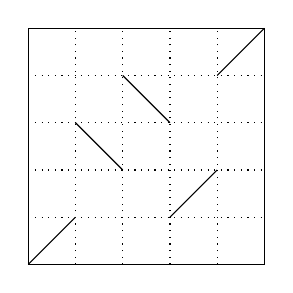
\begin{tikzpicture}[scale=.2]
        \draw[black] (0,0) -- (15,0) -- (15,15) -- (0,15) -- cycle;
        \foreach \i in {3,6,9,12}{
          \draw[dotted] (0, \i) -- (15, \i);
          \draw[dotted] (\i, 0) -- (\i, 15);
        }
        \draw (0,0) -- (3,3);
        \draw (12,12) -- (15,15);
        \draw (3,9) -- (6,6);
        \draw (6,12) -- (9,9);
        \draw (9,3) -- (12,6);

      \end{tikzpicture}
      \caption[The class of permutations which are at most two block reversals]{
      The class of permutations which are at most two block reversals
      from the identity is given by inflations of the four peg permutations
      $\pl 1 \mn 4 \pl 3 \mn 2 \pl 5$, $\pl 1 \mn 2 \pl 3 \mn 4 \pl 5$, 
      $\pl 1 \pl 4 \mn 2 \mn 3 \pl 5$, and $\pl 1 \mn 3 \mn 4 \pl 2 \pl 5$.}
      \label{polyclass:fig:twoblockrevs}
    \end{figure}
  

  \subsection{Data}
  
    Calculating the number of permutations of length $n$ which are at most $k$ operations
    away from the identity helps to understand how these block transformations
    differ, and how accurately they model biological mutation. The following
    tables show the numbers of these permutation in each radii from the
    identity, and build on the data presented in~\cite{GenomeBook}. The
    polynomials (in the variable $n$) enumerating these classes have integer
    coefficients when presented with the basis $\{\binom{n}{k}\}_{k \geq 0}$
    (as implied by~\cite{Klazar2003}). These enumerations are presented in the
    tables below. 
  

    \begin{table}[t]
    \caption{Number of permutations of length $n$ within $k$ block transpositions of the
              identity.}
    \begin{footnotesize}
    $$
    \begin{array}{rrrrrrrrrrrc} 
    k &\ 1\ &\ 2\ &\ 3\ &\ 4\ &\ 5\ &\
    6\ &\ 7\ &\ 8\ &\ 9\ &10&\text{\OEISref}\\\hline
    1&1&2&5&11&21&36&57&85&121&166&\text{\OEISlink{A000292}}\\[0.5ex]
    &\multicolumn{10}{c}{{n\choose 0}+{n\choose 2}+{n\choose 3}}&\\[1ex]
    2&1&2&6&23&89&295&827&2017&4405&8812&\text{\OEISlink{A228392}}\\[0.5ex]
    &\multicolumn{10}{c}{{n\choose 0}+{n\choose 2}+2{n\choose 3}+8{n\choose
    4}+18{n\choose 5}+11{n\choose 6}}&\\[1ex]
    3&1&2&6&24&120&675&3527&15484&56917&179719&\text{\OEISlink{A228393}}\\[0.5ex]
    &\multicolumn{10}{c}{\text{\scriptsize $\nc0 + \nc2 + 2\nc3 + 9\nc4 +
    44\nc5 + 220\nc6 + 656\nc7 + 841\nc8 + 369\nc9$} }&\\[1ex]
    \end{array}
    $$
    \end{footnotesize}
    \end{table}

    \begin{table}[t]
    \caption{Number of permutations of length $n$ within $k$ prefix transpositions of the 
    identity.}
    \begin{footnotesize}
    $$
    \begin{array}{rrrrrrrrrrrc}
    k &\ 1\ &\ 2\ &\ 3\ &\ 4\ &\ 5\ &\ 6\ &\ 7\ &\ 8\ &\ 9\
    &10&\text{\OEISref}\\\hline 1& 1& 2& 4& 7& 11& 16& 22& 29& 37&
    46& \text{\OEISlink{A000124}}\\[0.5ex]
    &\multicolumn{10}{c}{\nc0 + \nc2  }&\\[1ex]
    2& 1& 2& 6& 21& 61& 146& 302& 561& 961& 1546& \text{\OEISlink{A228394}}\\[0.5ex]
    &\multicolumn{10}{c}{\nc0 + \nc2  + 2\nc3 + 6\nc4 }&\\[1ex]
    3& 1& 2& 6& 24& 116& 521& 1877& 5531& 13939&
    31156&\text{\OEISlink{A228395}}\\[0.5ex]
    &\multicolumn{10}{c}{\nc0 + \nc2 + 2\nc3 + 9\nc4 + 40\nc5 + 90\nc6
    }&\\[1ex]
    \end{array}
    $$
    \end{footnotesize}
    \end{table}
  
    \begin{table}[t]
    \caption{Number of permutations of length $n$ within $k$ block reversals of the
    identity.}
    \begin{footnotesize}
    $$
    \begin{array}{rrrrrrrrrrrc}
    k &\ 1\ &\ 2\ &\ 3\ &\ 4\ &\ 5\ &\ 6\ &\ 7\ &\ 8\ &\ 9\
    &10&\text{\OEISref}\\\hline
    1&1&2&4&7&11&16&22&29&37&46&\text{\OEISlink{A000124}}\\[0.5ex]
    &\multicolumn{10}{c}{{n\choose 0}+{n\choose 2}}&\\[1ex]
    2&1&2&6&22&63&145&288&516&857&1343&\text{\OEISlink{A228396}}\\[0.5ex]
    &\multicolumn{10}{c}{8{n\choose 0}-3{n\choose 1}+{n\choose 2}+4{n\choose 3}}&\\[1ex]
    3&1&2&6&24&118&534&1851&5158&12264&25943&\text{\OEISlink{A228397}}\\[0.5ex]
    &\multicolumn{10}{c}{\text{ \scriptsize $318\nc0 -214\nc1 +131\nc2 -61\nc3
    +20\nc4 +70\nc5 +35\nc6$  }}&\\[1ex]\end{array}
    $$
    \end{footnotesize}
    \end{table}
  
    \begin{table}[t]
    \caption{Number of permutations of length $n$ within $k$ prefix reversals of the
    identity.}
    \begin{footnotesize}
    $$
    \begin{array}{rrrrrrrrrrrc}
    k &1&2&3&4&5&6&7&8&9&10&\text{\OEISref}\\\hline
    1&1&2&3&4&5&6&7&8&9&10&\text{\OEISlink{A000027}}\\[0.5ex]
    &\multicolumn{10}{c}{{n\choose 1}}&\\[1ex]
    2&1&2&5&10&17&26&37&50&65&82&\text{\OEISlink{A002522}}\\[0.5ex]
    &\multicolumn{10}{c}{2 \nc0 -1 \nc1 + 2\nc2  }&\\[1ex]
    3&1&2&6&21&52&105&186&301&456&657&\text{\OEISlink{A228398}}\\[0.5ex]
    &\multicolumn{10}{c}{ -3 \nc0 + 3 \nc1 - 2\nc2 + 6\nc3}&\\[1ex]
    \end{array}
    $$
    \end{footnotesize}
    \end{table}


    \begin{table}[t]
    \caption{Number of permutations of length $n$ within $k$ cut-paste moves of the
    identity.}
    \begin{footnotesize}
    $$
    \begin{array}{rrrrrrrrrrrc}
    k &1&2&3&4&5&6&7&8&9&10&\text{\OEISref}\\\hline
    1&1&2&6&16&35&66&112&176&261&370&\text{\OEISlink{A060354}}\\[0.5ex]
    &\multicolumn{10}{c}{\nc1 + 3\nc3 }&\\[1ex]
    2&1&2&6&24&120&577&2208&6768&17469&39603&\text{\OEISlink{A228399}}\\[0.5ex]
    &\multicolumn{10}{c}{-18\nc0 + 45\nc1 - 61\nc2 + 70\nc3 - 53\nc4 + 88\nc5
    + 107\nc6}&\\[1ex]
    3&1&2&6&24&120&720&5040&36757&223898&1055479&\text{\OEISlink{A228400}}\\[0.5ex]
    &\multicolumn{10}{c}{508264\nc0 - 280036\nc1 + 140012\nc2 - 57622\nc3 +
    13839\nc4}&\\[1ex]
    &\multicolumn{10}{c}{+ 4136\nc5-5368\nc6 + 531\nc7 + 21125\nc8 +
    12615\nc9} \\ 
    \end{array}
    $$
    \end{footnotesize}
    \end{table}
  

    \begin{table}[t]
    \caption{Number of permutations of length $n$ within $k$ block interchanges of the
    identity.}
    \begin{footnotesize}
    $$
    \begin{array}{rrrrrrrrrrrc}
    k &1&2&3&4&5&6&7&8&9&10&\text{\OEISref}\\\hline
    1&1&2&6&16&36&71&127&211&331&496&\text{\OEISlink{A145126}}\\[0.5ex]
    &\multicolumn{10}{c}{{n\choose 0}+{n\choose 2}+2{n\choose 3}+{n\choose
    4}}&\\[1ex]
    2&1&2&6&24&120&540&1996&6196&16732&40459&\text{\OEISlink{A228401}}\\[0.5ex]
    &\multicolumn{10}{c}{{n\choose 0}+{n\choose 2}+2{n\choose 3}+9{n\choose
    4}+44{n\choose 5}+85{n\choose 6}+70{n\choose 7}+21{n\choose 8}}&\\
    \end{array}
    $$
    \end{footnotesize}
    \end{table}


